\chapter{Iris wave guide for THz radiation transport}

    \section{Introduction}
    Incorporating a THz source at the European XFEL facility, utilizing a spent beam, would necessitate propagating the THz radiation from the location of the beam dump at XHE4/XS4 to the experimental hall of the users' end stations in XHQ, a distance estimated to be 370 meters, as seen in Fig.~\ref{Fig:transport outline}. Propagation of THz radiation over such a long distance imposes significant challenges, especially if the transmission system is required to accept a broadband of frequencies, spanning from $3$ to $30$ THz or even broader, down to $0.3$ THz.
    
    \begin{figure*}[h!]
    	\centering
    		\includegraphics[width=0.99\linewidth]{content/images/transport/aerial_view.pdf}
    		\centering
            \captionsetup{justification=centering}
        	\caption{Aerial view on the European XFEL campus with marking location of XHE4/XS4 and the users' hall in XHQ, the distance between them is measured to be $370$~m. In the call-out the scheme of XHE4/XS4 building at the UG2 level with outlined path of THz radiation through radiation protection maze. The diagnostic table is marked with a cyan blue rectangle}
        \label{Fig:transport outline}
    \end{figure*}
    
    THz radiation is highly absorbed by media and it is essential to avoid usage of any refractive optic elements, including filters and windows. To guide THz radiation one can consider using reflective optics or waveguides adjusted for the THz radiation range. The first approach, using reflective optics, is very suitable for complex tunnel geometries where one needs to guide radiation around corners. In contrast, waveguides are naturally suited to straight sections. In the THz radiation propagation beamline at the European XFEL, we plan to use both approaches: initial outcoupling occurs in XHE4/XS4, where radiation should be delivered to the XTD8 tunnel through a concrete radiation protection maze by means of a mirror-based system as illustrated in  the call-out in Fig.~\ref{Fig:transport outline}. And then we plan to deliver THz radiation through a $370$-meter-long XTD8 tunnel using a waveguide.
    
    In this chapter, we first provide an analysis of the THz radiation waveguide performance. We present two approaches to estimate its performance: one based on numerical simulation and the other using an analytical solution derived from complex boundary conditions. We calculate the efficiency of propagation of the fundamental mode of this waveguide and demonstrate the matching conditions for the incoming radiation. Additionally, we analyze the effects of imperfections on the waveguide's performance. Secondly, we outline the mirror-based propagation line and introduce a 'matching' device that ensures efficient coupling of the radiation from the source and the initial mirror system to the iris line.
    
    %\rr{discuss more about pros and cons of } Both approaches — one based on optical mirrors and the other on the iris line — have their advantages and limitations, and several considerations should be assessed before choosing one over the other. Mirrors offer a specific advantage in terms of achromaticity, allowing a mirror guide to be used across a wide range of frequencies. However, guiding a beam in a mirror system requires constant refocusing. The spacing between each refocusing section, which keeps the beam parallel, must be estimated by considering the Rayleigh length of the radiation to prevent divergence, as well as potential misalignment in the mirror setup. Large spacing may lead to significant deviations from the optical axis. Another consideration is the 45° incidence angle of the radiation on the mirrors, which means that a mirror-based system does not follow a straight line. In contrast, an iris line is inherently straight unless a bend is required, which can be achieved by inserting a plane mirror in the waveguide. The iris line also benefits from relatively low losses, around 10 \% per 100 meters of propagation, and is fairly tolerant to misalignment of the apertures, up to a scale of 1 mm. 

\section{Iris line theory}

    A waveguide for THz radiation consists of metallic screens with centered holes, as depicted in Fig.\ref{Fig:iris_mirror} (a). The 'virtual' side surface created by the screens effectively acts as a waveguide in the usual sense. We refer to this device as an iris line or an iris waveguide. The iris line actually bridges the gap between radio electronics and optics as it mixes the properties of usual waveguides using the theory of physical optics. The analysis of the electromagnetic field distribution in the iris line was first conducted using a numerical approach by Fox and Li\rr{cite}, followed by an analytical solution provided by Vainstein. Vainstein introduced complex boundary conditions at this virtual surface of the screen openings and derived the explicit expression of the iris line eigenmodes. Later, it was proposed~\rr{cite} to apply the iris line for THz radiation transportation at FEL facilities. The authors of~\rr{cite} present a comparative theoretical analysis of the iris line based on the theories of Fox and Li, and Vainstein, in application to the design of the transportation line. In this section, we extend the numerical approach further using an even simpler simulation approach that allowed us to account for the iris line imperfections. We also cross-checked our simulation results of the ideal iris line with the predictions given by Vainstein's theory and found excellent agreement.
    
    \begin{figure*}[h!]
    	\centering
    	% Answer: [trim={left bottom right top},clip]
    		\includegraphics[ width=0.79\linewidth]{content/images/transport/iris_mirror.pdf}
    		\centering
            \captionsetup{justification=centering}
        	\caption{Iris line and mirrors system outlines. Iris line has two main parameters: $a$ is the radius of the hole and $b$ is spacing between screens.}
        \label{Fig:iris_mirror}
    \end{figure*}
    
    As we mention, Fox and Li utilize a more numerical approach to finding the field distribution after radiation propagates through the iris line. This approach relies on the derivation of a radiation 'propagator' using physics optics. This implies that the iris line is essentially treated as a diffraction device, as depicted in Fig.~\ref{Fig:difraction_outline}. The first observation is that radiation incident on each screen will be partially diffracted back inside the virtual waveguide and partially inside the space between the screens. The latter portion of radiation will be reflected several times and will eventually be lost between two screens and does not affect the virtual waveguide. Therefore, Fox and Li made the primary approximation that the screen can be considered fully absorbing. 
    
    The second observation is that the problem can indeed be converted to the problem of radiation diffraction at an aperture. In this case, the Fresnel number is the only dimensionless parameter needed to describe the problem: $N = a^2 / (\lambda b)$, where $a$ is the radius of the opening of the iris line screens, $b$ is the spacing between screens, and $\lambda$ is the radiation wavelength. Comparing the approaches of Fox and Li and Vainstein's approach, one can see that namely, $N$ describes the transmission efficiency of the iris line, which we will show later in this section. For our simulations, we implemented the simplified Fox and Li approach. We propagate radiation in free space from the location of the $n$-th screen to the $(n+1)$-th screen and then apply a fully absorbing aperture, after which we repeat the propagation procedure again for the next cell.
    \begin{figure}[h!]
    	\centering
    		\includegraphics[trim={0 5cm 0 0cm}, width=0.75\linewidth]{content/images/transport/difraction_outline.jpeg}
    		\centering
            \captionsetup{justification=centering}
        	\caption{Iris line and mirrors system outlines}
        \label{Fig:difraction_outline}
    \end{figure}
    
    The approach developed by Vainstein, is mathematically robust and addresses the problem by taking into account the boundary conditions of the metallic walls and screens of the iris line: 
    
    \begin{align}
        \left[\vec{\widetilde{E}}+ (1+i) \beta_0 \sqrt{c b/(4 \omega)} ~
        (\vec{n} \cdot \vec{\nabla}_\bot) \vec{\widetilde{E}}\right]_{S} =
        0, 
        \label{Eq:Vainstein}
    \end{align}
    
    where $S$ is the virtual surface formed by the screens of the iris line, and
    $\vec{n}$ is the unit vector normal to $S$, $\beta_0 = 0.824$, $c$ is the speed of light, $\omega$ is the radiation frequency and $\widetilde{E}(r,\phi,z)$ is the amplitude.

    We seek the solution for the field amplitude, $\widetilde{E}(r,\phi,z)$, in the following form:
    
    \begin{align}
        \widetilde{E} = u_{nj}(r)\exp[-in \phi -i k_z z]~, \label{solu}
    \end{align}

    where $n = 0,1, 2, ...$ and $u_{nj}(r)$ should be solution of the following homogeneous equation as we consider axially symmetric iris line:
    
    \begin{align}
        r^2 u_{nj}'' + r u_{nj}' + [(k_{nj})^2 - n^2)] u_{nj} = 0~,
        \label{homogeq}
    \end{align}
    
    and after substituting $\widetilde{E}(r,\phi,z)$ in Eq.~\ref{Eq:Vainstein} we obtain boundary condition on $u_{nk}(r)$ in the following form:
    
    \begin{align}
        [u_{nj} + (1+i) \beta_0 \sqrt{c b/ (4\omega)} u_{nj}']_{r = a} = 0.
        \label{boundh}
    \end{align}
    
    assuming $N \gg 1$ we write the functions $u_{nj}$ in the form:
    
    \begin{eqnarray}
        u_{nj} = J_n(k_{nj} r)
        \label{Eq:Bessel}
    \end{eqnarray}

    where
    
    \begin{eqnarray}
        k_{nj} = \frac{\nu_{nj}}{a} [1-(1+i) \beta_0 M], 
        \label{Eq:k_nj}
    \end{eqnarray}
    
    and $\nu_{nj}$ is the $j$-th root of the $n$-th order Bessel
    function of the first kind ($J_n(\nu_{nj}) = 0$), and $M = (8 \pi N)^{-1/2}$. Substituting Eq.~\ref{Eq:k_nj} into the dispersion relation:
    
    \begin{eqnarray}
        k_z^2 + k_{nj}^2 = \frac{\omega^2}{c^2},
        \label{kzzz}
    \end{eqnarray}

    we obtain:
    
    \begin{eqnarray}
        k_z b = \frac{\omega b}{c} - 2 \nu_{nj}^2 M^2 + 4 \nu_{nj}^2 M^3
        (1+i)\beta_0. 
        \label{kzzz2}
    \end{eqnarray}
    taking the imaginary part from this we can find the radiation power losses per transit of one iris as:
    
    \begin{eqnarray}
        2 \mathrm{Im}(k_z b) = 8 \nu_{nj}^2 M^3 \beta_0. 
        \label{loss}
    \end{eqnarray}
    
    The relative loss of the $j$-th mode of order $n$ after traveling
    for a distance $z$ is therefore given by
    
    \begin{eqnarray}
    \left(\frac{\Delta W}{W}\right)_{nj} = 1- \exp\left(-\frac{
    \nu_{nj}^2\beta_0  }{ (2\pi N)^{3/2}}\frac{z}{b}\right) = 1-
    \exp\left(-\frac{ \nu_{nj}^2\beta_0 (\lambda b)^{3/2} }{
    (2\pi)^{3/2} a^3}\frac{z}{b}\right)~.\label{loss}
    \end{eqnarray}
    
    As one can see, lower-order modes tend to survive, showing a weak dependency on the spacing between the irises, denoted by $b$, and a much stronger dependence on $\lambda$ and $a$. These results provide an analytical basis for cross-checks with the numerical approach based on physical optics.
    
    
    This leads to a definitive expression for the fundamental mode, denoted as $u_{nj}$.
    
    \begin{align}
        u_{nj} = J_n(k_{nj} r),
        \label{Eq:mode_shape}
    \end{align}
    where $k_{nj} = \cfrac{\nu_{nj}}{a} \bigg(1 - (1 + i)\beta_0 M \bigg)$ and $\nu_{nj}$ is the $j$-th root of the $n$-th order Bessel function of the first kind, e.g. $J_n(k_{nj}) = 0$. $M = (8 \pi N)^{-1/2}$ and $\beta_0 = 0.824$. And relative loss of the $j$-th mode of order $n$-th after propagation over $z$ meters:
    
    \begin{align}
        \bigg(\cfrac{\Delta W}{W} \bigg)_{nj} = 1 - \exp{\bigg[ -\frac{\nu^2_{nj}\beta_0}{(2 \pi N)^{3/2}} \cfrac{z}{b} \bigg]} = 1 - \exp{\bigg[ -\frac{\nu^2_{nj}\beta_0 (\lambda b)^{3/2}}{(2 \pi)^{3/2} a^3} \cfrac{z}{b} \bigg]}.
        \label{Eq:Losses_in_iris_line}
    \end{align}
    

\section{Analysis of 3 THz radiation propagation}
    
    In this section, we present the results of propagating $3$ THz radiation through the iris line. Studying the iris line at the lowest radiation frequency is justified by the fact that, the higher the radiation frequency, the better the radiation transmission performance of the iris line, as can be seen from Eq.~\ref{Eq:Losses_in_iris_line} or through the visual representation of this equation given in Fig.\ref{Fig:mode_losses}. We examine the performance of the iris line with a numerical approach and cross-check both the level of radiation losses according to Eq.~\ref{Eq:Losses_in_iris_line} and the spatial radiation distribution given by Eq.~\ref{Eq:Bessel}. 
    
    \begin{figure}[h!]
    	\centering
    		\includegraphics[trim={0 0cm 0 0cm}, width=0.99\linewidth]{content/images/transport/plane_wave.png}
    		\centering
            \captionsetup{justification=centering}
        	\caption{Result of a plane wave propagation thought an iris line. Subplot in the upper right represent a line of the intensity distribution of the radiation. The black dashed line represent relative loss of the radiation per cell and the red line show the portion of radiation left at the give distance from the entrance.}
        \label{Fig:plane_wave}
    \end{figure}
    
    At first we study the eigenmodes of the iris line by propagating a plane wave through it, as plane wave encompasses all possible modes. With this simulation we observe that only the fundamental mode will remain after sufficiently long propagation distance, as indicated by Eq.\ref{Eq:Losses_in_iris_line}. This way we can demonstrate that the numerical approach coincides with the analytical expression given by Eq.~\ref{Eq:mode_shape}. Moreover, with this we show the mode filtering mechanism happening in the iris line. In Fig.\ref{Fig:plane_wave} we show in the right upper subplot the resulting Gaussian-like intensity distribution that actually follows Eq.~\ref{Eq:mode_shape} as we illustrate in Fig.~\ref{Fig:comparison_spatial_dist}. we set the preliminary design parameters of the iris line: $a = 0.055$~m and $b = 0.3$~m, that corresponds to $N = 101$.
    
    The oscillating behavior in the relative losses per cell is happening due to the fact that, even after $900$ m of propagation, there is a mixture of higher modes, predominantly the second mode, that are still present, which can be seen in Fig.~\ref{Fig:mode_losses}.

    \begin{figure}[h!]
        \centering
        \begin{minipage}{0.45\textwidth}
            \centering
            \includegraphics[width=\textwidth]{content/images/transport/prop_losses_Nf_101_z_370.pdf} % First image
            \caption{Analytical estimation of the radiation losses in the iris line.}
            \label{Fig:mode_losses}
        \end{minipage}\hfill
        \begin{minipage}{0.45\textwidth}
            \centering
            \includegraphics[width=\textwidth]{content/images/transport/mode_vs_prop.pdf} % Second image
            \caption{The radiation intensity distribution at the exit of the iris line.}
            \label{Fig:comparison_spatial_dist}
        \end{minipage}
    \end{figure}
    
    Comparing the shape of the field distribution obtained from numerical simulations, there are minor differences relative to what is predicted by Vainstein's theory in Eq.~\ref{Eq:mode_shape}. The oscillating features indicate that the numerical approach accounts for higher-order diffraction, while Vainstein's theory considers contributions only from the first diffraction order. The same results are presented in~\rr{cite}.
    
    \begin{figure}[h!]
    	\centering
    		\includegraphics[trim={0 0cm 0 0cm}, width=1.\linewidth]{content/images/transport/iris_mode.png}
    		\centering
            \captionsetup{justification=centering}
        	\caption{Result of a fundamental mode propagation thought an iris line. Relative losses per cell is constant, spatial radiation distribution is perfectly preserved along the waveguide.}
        \label{Fig:iris_mode}
    \end{figure}
    
    And secondly, we study the transmission efficiency of the fundamental mode. We present the flawless propagation of the fundamental mode in Fig.~\ref{Fig:iris_mode}, where the relative loss at each iris line cell is constant and is at the level of $0.03 \%$, and the spatial distribution of the radiation is preserved. This estimation of relative loss per cell is in very good agreement with Eq.~\ref{Eq:Losses_in_iris_line}. Utilizing the fundamental mode for radiation transport in the iris line is highly preferable, although it necessitates a careful solution to the mode matching problem when in coupling to the iris line.
    
\subsection{In-coupling condition}
    
    The geometry of the iris line imposes specific requirements on the incoming radiation: the iris line will filter out all radiation that arrives at angles greater than $a/(bN)$, which practically means that the incoming beam should be parallel. Another requirement for the radiation distribution is that it should be as close as possible to the distribution of the fundamental mode given by Eq.~\ref{Fig:iris_mode}. Obviously, achieving a perfect Bessel function distribution for the input radiation of the iris line is not always feasible. Most importantly, it is essential to provide an approximation that is good enough to fit this Bessel distribution with a given bell-like distribution and then empirically manipulate its width to achieve the highest possible output from the iris line. For example a model Gaussian distribution with optimised width of $\sigma = a / 2.85$ has $67.8 \%$ radiation power left after $370$~m of propagation, which is compared to the fundamental mode losses ($69.2 \%$) is a very decent result. 
    
    %flattop $52.3 \% (can be seen from fig 7.5)$

\subsection{Optimization of iris line dimensions for $0.3 - 30$~THz radiation propagation}
\label{Sec:Optimization of iris line dimensions for 0.3 - 30 THz radiation propagation}
    Extending the frequency band from $3 - 30$~THz down to $0.3$~THz will necessitate changes to the dimensions of the iris line to ensure sufficient enough efficiency at lower frequencies. Primarily, the radius $a$ should be adjusted and $b$ can be left unchanged. 
    \begin{figure}[h!]
    	\centering
    		\includegraphics[trim={0 0cm 0 0cm}, width=0.55\linewidth]{content/images/transport/power_left4a.pdf}
    		\centering
            \captionsetup{justification=centering}
        	\caption{Transmission efficiency with different radii with respect to frequency.}
        \label{Fig:power_left4a}
    \end{figure}  
    As indicated by Eq.\ref{Eq:Losses_in_iris_line}, the radius significantly influences the transmission performance of the iris line. In Fig.\ref{Fig:power_left4a}, we illustrate the transmission of the iris line over a $370$ m propagation distance for the entire $0.3 - 30$ THz frequency band. The choice of an appropriate radius should be based on the technical feasibility of manufacturing such a long device within specified tolerances.

\subsection{Wave packet enlargement}

    Up to now, we have simulated the propagation of monochromatic, spatial radiation distributions to study the effect of the iris line on the radiation distribution at a given radiation wavelength. In reality, the entire wave packet will be propagated. We have examined this issue both analytically and numerically. Numerical simulations have not shown any affect in the time and frequency domain distributions, except for the expected attenuation that depends on the radiation wavelength.
    %\rr{include analytical derivation}\\ 
    %\oo{it does make much sense to include simulations}
    
\subsection{Tolerances estimation}

    Building an iris line can present significant technical challenges due to its length and the overall number of iris screens required. In this section, we discuss the precision necessary for manufacturing and assembling each iris screen to ensure the transmission efficiency of the entire waveguide. As previously discussed, the iris line operates primarily on the principle of diffraction: each aperture acts as an obstacle, scattering half of the radiation back into the body of the waveguide, and the other half outward into the open cavity of the iris line. This design minimizes Ohmic losses, which are inevitable when radiation encounters the metallic walls, the only losses occurring is due to the portion of radiation diffracted outward from the virtual waveguide. Most importantly is that these losses are determined geometrically: any misalignment of the irises or errors in the size of the iris openings can result in the 'cutting' of an additional portion of radiation compared to the ideally aligned case, thereby increasing losses.
    \begin{figure}[h!]
    	\centering
    		\includegraphics[trim={0 0cm 0 0cm}, width=0.55\linewidth]{content/images/transport/losses.pdf}
    		\centering
            \captionsetup{justification=centering}
            \caption{Blue circles correspond to iris radius size errors, orange crosses to the misplacement of irises in the $x$ direction only, and green circles display misplacement in both the $x$ and $y$ directions. Red squares correspond to uneven spacing between irises, while rhombuses represent the cumulative losses accounting for all effects, with corresponding values of the misplacements.}  
            \label{Fig:losses}
    \end{figure}
    
    We studied the performance of a non-ideal iris line by propagating the fundamental mode. Our investigation included introducing errors in iris radius size, misalignments in the transverse plane (only in one direction and both directions), and the influence of small, non-periodic placements of the irises along the line. We then simulated the performance of the iris line, taking into account all the aforementioned misalignments. 
    
    The results of this simulation are presented in Fig.~\ref{Fig:losses}, where we show the relative losses per cell in relation to the magnitude of misplacement. Assuming that the errors follow a Gaussian distribution in amplitude, we simulated the propagation of the fundamental mode through 300 irises for each data point and then calculated the average relative loss per cell. An estimation of the fraction of radiation remaining after 370 meters of propagation can be made using the following expression: $e^{-\epsilon n} = 0.603$, where $\epsilon$ is taken from Fig.~\ref{Fig:losses} and $n$ is number of screens. Here we assumed that tolerances are at the level of $0.75$ mm, where $n$ is the number of irises, calculated as $n = L/b$.
    \begin{figure}[h!]
    	\centering
    		\includegraphics[trim={0 0cm 0 0cm}, width=0.65\linewidth]{content/images/transport/disp_plot.pdf}
    		\centering
            \captionsetup{justification=centering}
        	\caption{Modeled misalignments of the irises accounting for the overall bends of the line.}
        \label{Fig:disp_plot}
    \end{figure}
    \begin{figure}[h!]
    	\centering
    		\includegraphics[trim={0 0cm 0 0cm}, width=1.\linewidth]{content/images/transport/prop_misalighments.png}
    		\centering
            \captionsetup{justification=centering}
        	\caption{Propagation of the fundamental mode through a non-ideal iris line taking into account misalignments of the screens, the overall bend of the line, errors in the iris radius openings, and uneven spacing between the screens, as depicted in~\ref{Fig:disp_plot}.}
        \label{Fig:iris_mode}
    \end{figure}
    One can see that the dependence is quadratic-like, which is explainable since the losses are solely due to diffraction in this model and scale proportionally to the area blocked by the iris screen.
    
    We include overall bends of the iris line in the simulations. In Fig.~\ref{Fig:disp_plot} we present the misalignment of if each individual iris overlaid with adiabatic bend of the the whole line, which we assumed to be nearly harmonic for this model example. We accounted two types of the bends with low frequency and with higher oscillations that one can see in $y$ direction in the Fig.~\ref{Fig:disp_plot}. This higher oscillatory behaviour may occur in between two stands that support the metallic tube of the iris line due to its own weight. 
    
    In principal the magnitude of this bands should be smaller than irises misplacements to have no effect on the wave guide performance. We estimated that tolerable amplitude of the bend is at the level of $2$~mm. We presented results of the propagation of the fundamental mode in Fig.~\ref{Fig:disp_plot}, which result in nearly $4 \%$ power drop at the output with respect to the non-bended case.
    
    \subsection{Razor-edge taper of iris screens}
    \oo{Will be contributed by Adham E. Naji}\\
    \rr{the text below is to be deleted}\\
    \begin{figure}[h!]
    	\centering
    		\includegraphics[trim={0 0cm 0 0cm}, width=0.45\linewidth]{content/images/transport/cutting_edge.pdf}
    		\centering
            \captionsetup{justification=centering}
        	\caption{Cutting edge of the iris opening}
        \label{Fig:cutting_edge}
    \end{figure}
    \rr{As demonstrated, the mathematical model of an iris line is based on diffraction effects and the approximation of infinitesimally thin irises. In reality, the thickness of actual screens can vary by a few millimeters, introducing contributions from Ohmic losses. Interestingly, to some extent, an increase in screen thickness can reduce diffraction losses, as illustrated in~\ref{Fig:cutting_edge}. However, finding a trade-off in thickness poses significant theoretical and technical challenges. To mitigate this issue and achieve a fully controlled system, one strategy involves sharpening the screen edges, as proposed in Fig.~\ref{Fig:cutting_edge}. This approach minimizes interaction with the screen's end face. cite~\rr{A. Naji}}
    
\section{THz delivery to the diagnostics table and in-coupling to the iris line}

    Before entering the iris line, the beam should be delivered through a concrete maze to the room where the diagnostic table will be located, as shown in Fig.~\ref{Fig:mirrors_outline}. To address this, a mirror-based system can be used to guide the radiation. Mirrors placed at $45^\circ$ angles will facilitate guiding the radiation around corners.
    
    \begin{figure}[h!]
    	\centering
    		\includegraphics[trim={0 0cm 0 0cm}, width=0.99\linewidth]{content/images/transport/mirrors_outline.pdf}
    		\centering
            \captionsetup{justification=centering}
        	\caption{Scheme of the mirror delivery line to the diagnostic table in XHE4/XS4 building. Focusing mirrors are shown with curved black lines, circles with dot and cross inside indicate a periscope arraignment of the mirrors.}
        \label{Fig:mirrors_outline}
    \end{figure}
    
    We plan to use sections reminiscent of a Keplerian telescope, with equal focusing distances, in combination with 'straight' sections, as depicted in Fig.~\ref{Fig:mirrors_outline}. An alternative strategy could involve expanding the beam at the outset to achieve a large Rayleigh number, resulting in a highly collimated beam. However, this approach would necessitate a more precise mirror alignment to steer the beam accurately. The system we present here mitigates this issue. Nevertheless, there is potential for further optimization and modification of the optical system. Another requirement that the entire delivery line system should be mounted high enough to ensure it does not obstruct staff movement through the concrete maze, so we marking two periscopes in Fig.~\ref{Fig:mirrors_outline}.

    \subsection{Design of a beam expander}

    The second part of the problem involves constructing a beam expander, which also should be design using reflective optics to avoid the excessive absorption of radiation that would occur with refractive optics. This device is intended to expand the beam to the size that matches the iris's opening, minimizing transmission losses in the iris line as we described in the Sec.~\ref{Sec:Optimization of iris line dimensions for 0.3 - 30 THz radiation propagation}. Furthermore, the beam expander should be afocal, meaning that incoming and outcoming radiation is collimated. Also the system should be zoomable assuring a constant output radiation width while the incoming radiation may vary. The principal design of such a device requires three functional optical elements: focusing and defocusing elements, as described in~\rr{cite}. Fig.~\ref{Fig:Zoomlens} illustrates one of the possible solutions, referred in~\rr{cite} as the $(+-+)$ solution.
    \begin{figure}[h]
    	\centering
    		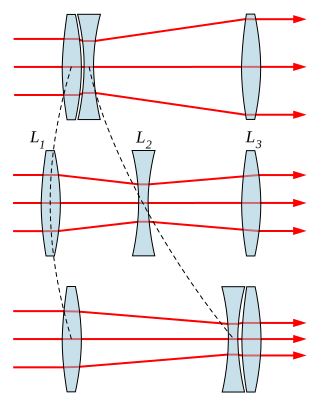
\includegraphics[trim={0 0cm 0 0cm}, width=0.45\linewidth]{content/images/transport/Zoomlens.pdf}
    		\centering
            \captionsetup{justification=centering}
        	\caption{An afocal zoom system with three optical elements, as depicted in the image taken from \rr{cite}. In a real mirror-based system, additional plane mirrors are included to enable adjustments in the distance between the (de)focusing elements and to direct the beam from the diagnostic table towards the iris line.}
        \label{Fig:Zoomlens}
    \end{figure}
    
    We outlined a mirror-based analogue of the beam expander, as presented in Fig.~\ref{Fig:beam_expander}. The combination of focusing/defocusing mirrors and plane mirrors is arranged in three blocks: $L_1$, $L_2$, and $L_3$. These blocks movable to be able to adjust the distance between the optical elements $D_1$ and $D_2$ independently and accommodate the zoom function of the device.
    \begin{figure}[h]
    	\centering
    		\includegraphics[trim={0 0cm 0 0cm}, width=0.99\linewidth]{content/images/transport/beam_expander.pdf}
    		\centering
            \captionsetup{justification=centering}
        	\caption{Conceptual design of a mirrors-based beam expander. $D_1$ and $D_2$ denotes distance between the first and the second one functional optical element and the second and the third one correspondingly. Plane mirror $p_3$ should be able pitch and roll as well as to be movable in $x$ and $y$ with respect to the optical axis of the iris line.}
        \label{Fig:beam_expander}
    \end{figure}
    The third plane mirror, $p_3$, should be adjustable to be able to align the optical axis of the beam expander with the iris line. This alignment can be achieved by adjusting the mirror's pitch and roll angles, as well as its $\Delta x$ and $\Delta y$ positions relative to the optical axis of the iris line.
    
\section{Conclusion}
    
    In this section, we discussed the systems designed for the propagation of THz radiation, aimed at delivering light pulses from XHE4/XS4 to the experimental hall of the European XFEL XHQ. The delivery system is comprised of three main components: the iris line, the mirror-based guiding line, and the afocal beam expander. The mirror-based guiding line facilitates the initial out-coupling of radiation from the source, guiding it to a diagnostic table. Following this, the afocal beam expander is used to match the outgoing radiation after diagnostic table, with the input requirements of the iris line, ensuring efficient transmission to the experimental hall. And finally, The iris line is responsible for transmitting radiation from the XHE4/XS4 through a 370-meter-long XTD8 tunnel.
    
    The mirror system comprises a primary 'catch' mirror designed to capture all radiation emitted from the Cherenkov waveguide and direct this radiation through a diamond window. Subsequently, the radiation is collimated by a second mirror. Downstream optics, positioned before the diagnostic table, will consist of alternating refocusing telescopes and 'straight' sections. This arrangement is intended to address alignment issues with the mirrors, ensuring that the radiation is efficiently delivered to the diagnostic table before being transferred to the beam expander.
    
    The beam expander must be afocal, ensuring that both the input and output radiation are collimated. The optical system should be designed to allow variations in the input waist size of the radiation without affecting the nearly constant output size. Additionally, it should be possible to adjust the output size in small increments to achieve optimal matching with the iris line for various radiation profiles.
    
    The iris line is capable of transmitting a broad range of frequencies, and its efficiency can be optimized by adjusting the dimensionless parameters, denoted as $N = a^2/(\lambda b)$. The transmission coefficient of the iris line is influenced by the radiation frequency and the structure of the line. For instance, an ideal iris line with $N = 101$ can achieve a transmission efficient at level of $0.69$ after $370$ m of propagation when the \textit{fundamental} mode is propagation through it. However, imperfections such as screens opening size errors, centering misalignments, and spacing between iris screens (RMS is $0.75$~mm), as well as overall bends in the line (RMS is $1.5$~mm), drop efficiency down to $0.56$. A key assumption in this study is that the input to the iris line matches its fundamental mode as close as possible. We have explored the performance of the iris line with inputs that differ from its fundamental mode using Gaussian distribution, and determined the optimal widths for in coupling of this distributions into the line. 
    